\chapter{Experiments}
\label{cha:6th_chapter}
This chapter describes the experiments we conducted in order to understand how the information is processed by the \ac{GAN}s implemented: in particular the focus was to investigate how the information passes through the generator network during the generative process.
Section \ref{sec:skip_analysis} contains a detailed study about the skip connections  while in Section \ref{sec:internal_analysis} we describe the analysis performed to observe the internal connections behaviour in the generator. In Section \ref{sec:experiments_discussion} we discuss the results.

We performed the experiments using the models trained to generate $T_{2flair}$. The results shown in this chapter are relative to the analyses of the MI-pix2pix generator network (since MI-p2p was the most competitive model in the synthesis of $T_{2flair}$). Further results from the experiments with pix2pix and MI-GAN can be found in Appendix \ref{cha:first_appendix}.

\section{Skip Connections Analysis}
\label{sec:skip_analysis}
Two experiments were performed in this section: in the first one (Subsection \ref{subsec:skips_turned_off}) we observed what happens to the output of the generator by sequentially turning off the skip connections (setting all the values in the skips to 0), from the innermost to the outermost and viceversa, while in the second experiment (Subsection \ref{subsec:skips_perturbed}) we replaced, again sequentially, the information passing through the skips of our analysed generator, with input image $A$, with the content from the skips of another generator, with input $B$ (where $A$ and $B$, from the same modality, belong to different subjects). 

\vspace{5mm}
Quantitative and qualitative results of the first experiment are presented in Table \ref{tab:quantitative_channels_off_mip2p} and Figure \ref{fig:qualitative_channels_off_mip2p} (where [1,1,1,1,0,0,0] means that the three outermost skip are off). Results from the second one are reported in Table \ref{tab:quantitative_channels_perturbed_mip2p} and Figure \ref{fig:qualitative_channels_perturbed_mip2p} where the configuration [AAAABBB] indicates that the generator was perturbed with image B in the three outermost skip connections.

Figure \ref{fig:config_skips} illustrates the setting in which the three outermost skip connections are turned off/perturbed (these connections are shown in red color), corresponding to the configurations mentioned above ([1,1,1,1,0,0,0]/[AAAABBB]).

\begin{figure}[H]
\centering
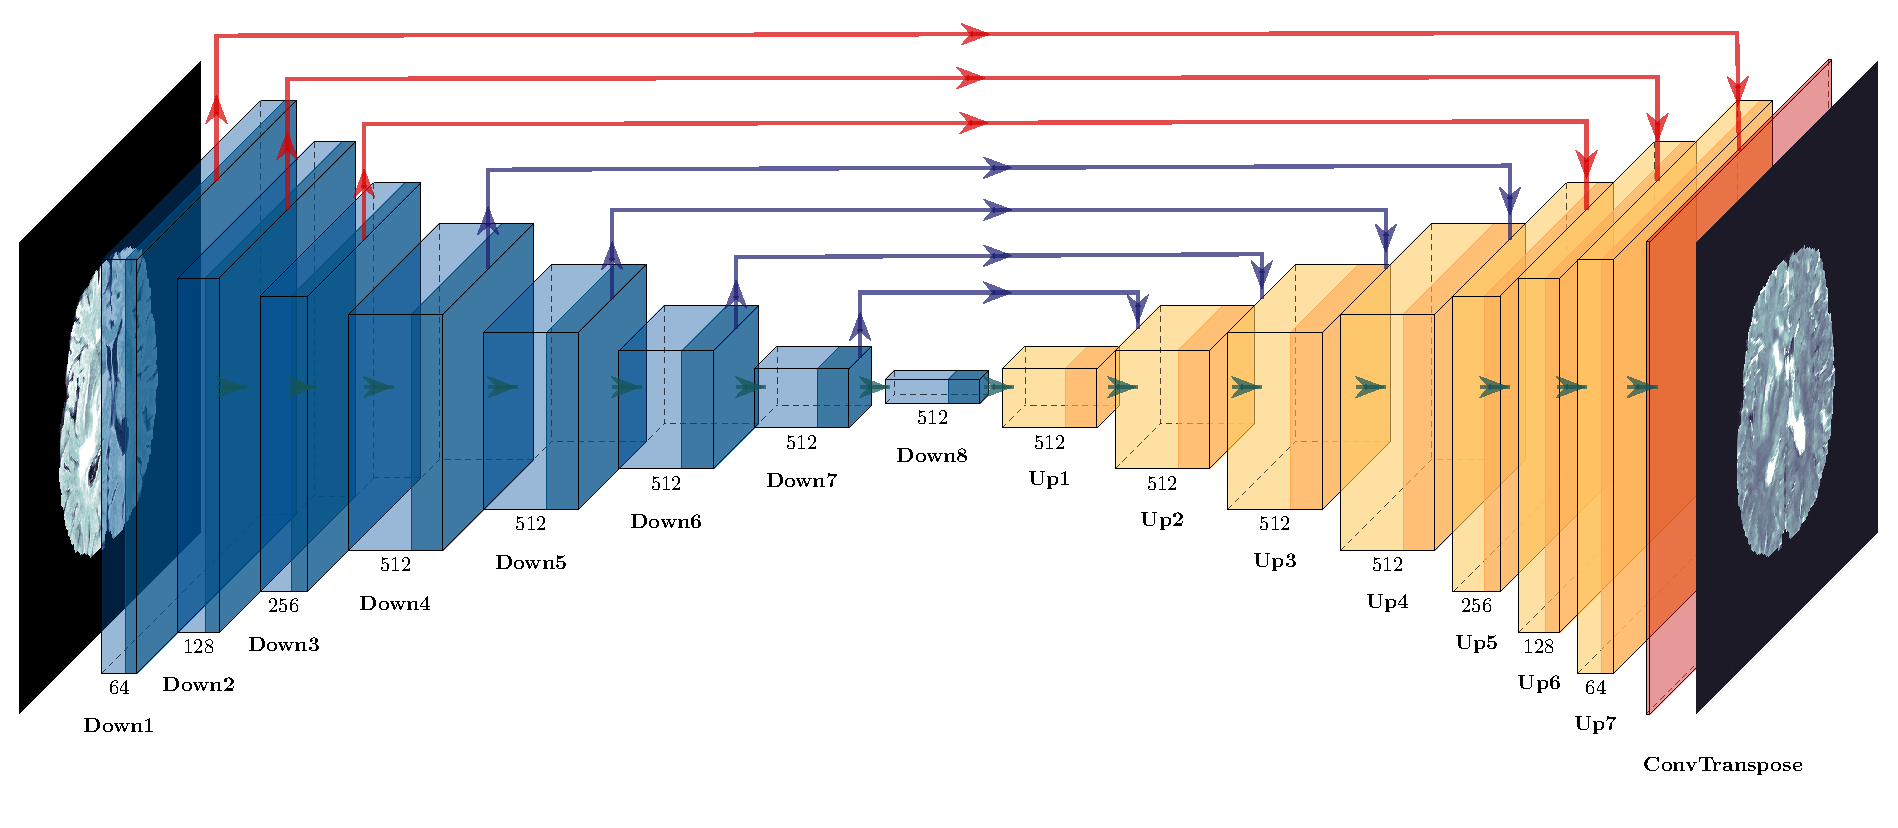
\includegraphics[height=0.266\textheight]{images/config_skips.pdf}
\caption[Configuration example in Skip Connections Analysis]{Example of network with the three outermost skip connections turned off/perturbed, corresponding to the configurations [1,1,1,1,0,0,0]/[AAAABBB].}
\label{fig:config_skips}
\end{figure}


%%%%%%%%%%%%%%%%  Channels off MI-p2p

\subsection{Channels Turned Off}
\label{subsec:skips_turned_off}
\begin{table}[H]
\centering
\fontsize{8.5}{16}\selectfont
\setlength{\tabcolsep}{4pt}
\begin{tabular}{l|c|c|c|c|c}
\toprule
\textbf{Skips off} & \textbf{MSE} & \textbf{PSNR} & \textbf{SSIM} & $\mathbf{MSE_{tumor}}$ & $\mathbf{PSNR_{tumor}}$\\
\hline

[1,1,1,1,1,1,1] & $\mathbf{0.0069\pm0.0049}$ & $\mathbf{22.8165\pm3.7317}$  & $\mathbf{0.7772\pm0.1094}$ & $\mathrm{0.0221\pm0.0375}$ & $\mathrm{19.0374\pm4.1582}$\\

[0,1,1,1,1,1,1] & $\mathrm{0.0071\pm0.0048}$ & $\mathrm{22.6609\pm3.7374}$  & $\mathrm{0.7718\pm0.1126}$ & $\mathbf{0.0209\pm0.0356}$ & $\mathbf{19.1225\pm4.0804}$\\

[0,0,1,1,1,1,1] & $\mathrm{0.0093\pm0.0053}$ & $\mathrm{21.3752\pm3.7214}$  & $\mathrm{0.7520\pm0.1163}$ & $\mathrm{0.0381\pm0.0251}$ & $\mathrm{14.8111\pm2.3423}$\\

[0,0,0,1,1,1,1] & $\mathrm{0.0103\pm0.0061}$ & $\mathrm{20.8808\pm3.6404}$  & $\mathrm{0.7217\pm0.1309}$ & $\mathrm{0.0374\pm0.0438}$ & $\mathrm{15.5332\pm3.1803}$\\

[0,0,0,0,1,1,1] & $\mathrm{0.0105\pm0.0059}$ & $\mathrm{20.8179\pm3.7360}$  & $\mathrm{0.7423\pm0.1175}$ & $\mathrm{0.0419\pm0.0235}$ & $\mathrm{14.3061\pm2.2416}$\\

[0,0,0,0,0,1,1] & $\mathrm{0.0147\pm0.0080}$ & $\mathrm{19.2806\pm3.4188}$  & $\mathrm{0.6610\pm0.1090}$ & $\mathrm{0.0779\pm0.0231}$ & $\mathrm{11.3254\pm1.6623}$\\

[0,0,0,0,0,0,1] & $\mathrm{0.0116\pm0.0060}$ & $\mathrm{20.1027\pm2.8014}$  & $\mathrm{0.5940\pm0.1035}$ & $\mathrm{0.0501\pm0.0212}$ & $\mathrm{13.3909\pm1.9644}$\\

[0,0,0,0,0,0,0] & $\mathrm{0.0987\pm0.0319}$ & $\mathrm{10.3797\pm1.8937}$  & $\mathrm{0.0202\pm0.0267}$ & $\mathrm{0.3230\pm0.1115}$ & $\mathrm{5.1401\pm1.4091}$\\
\hline
[1,1,1,1,1,1,1] & $\mathbf{0.0069\pm0.0049}$ & $\mathbf{22.8165\pm3.7317}$  & $\mathbf{0.7772\pm0.1094}$ & $\mathbf{0.0221\pm0.0375}$ & $\mathbf{19.0374\pm4.1582}$\\

[1,1,1,1,1,1,0] & $\mathrm{0.0105\pm0.0070}$ & $\mathrm{20.8009\pm3.3278}$  & $\mathrm{0.7434\pm0.1150}$ & $\mathrm{0.0332\pm0.0556}$ & $\mathrm{17.3071\pm4.3356}$\\

[1,1,1,1,1,0,0] & $\mathrm{0.0533\pm0.0256}$ & $\mathrm{13.4927\pm3.1335}$  & $\mathrm{0.3956\pm0.1498}$ & $\mathrm{0.1087\pm0.0973}$ & $\mathrm{10.8014\pm3.0530}$\\

[1,1,1,1,0,0,0] & $\mathrm{0.0846\pm0.0320}$ & $\mathrm{11.1146\pm1.9886}$  & $\mathrm{0.1106\pm0.0700}$ & $\mathrm{0.2253\pm0.1313}$ & $\mathrm{7.0131\pm2.0886}$\\

[1,1,1,0,0,0,0] & $\mathrm{0.0978\pm0.0336}$ & $\mathrm{10.4303\pm1.8611}$  & $\mathrm{0.0413\pm0.0491}$ & $\mathrm{0.3125\pm0.1390}$ & $\mathrm{5.3861\pm1.6662}$\\

[1,1,0,0,0,0,0] & $\mathrm{0.1050\pm0.0333}$ & $\mathrm{10.0808\pm1.7531}$  & $\mathrm{0.0134\pm0.0411}$ & $\mathrm{0.3362\pm0.1386}$ & $\mathrm{5.0176\pm1.5175}$\\

[1,0,0,0,0,0,0] & $\mathrm{0.0963\pm0.0315}$ & $\mathrm{10.4584\pm1.7412}$  & $\mathrm{0.0255\pm0.0419}$ & $\mathrm{0.3061\pm0.1227}$ & $\mathrm{5.4125\pm1.4862}$\\

[0,0,0,0,0,0,0] & $\mathrm{0.0987\pm0.0319}$ & $\mathrm{10.3797\pm1.8937}$  & $\mathrm{0.0202\pm0.0267}$ & $\mathrm{0.3230\pm0.1115}$ & $\mathrm{5.1401\pm1.4091}$\\
\midrule
\end{tabular}
\caption[Quantitative results from turning off the skips in MI-pix2pix]{Quantitative results from the Skip Connections Analysis on MI-P2P{$_{T_{2flair}}$}: skips are sequentially turned off.}
\label{tab:quantitative_channels_off_mip2p}
\end{table}

\begin{figure}[H]
\centering
\includegraphics[width=0.635\textheight]{images/skips_m2p.pdf}
\caption[Qualitative results from turning off the skips in MI-pix2pix]{Qualitative results from the Skip Connections Analysis on MI-P2P{$_{T_{2flair}}$}: skips are sequentially turned off. \textit{Prediction} corresponds to config.[1111111]}
\label{fig:qualitative_channels_off_mip2p}
\end{figure}

%\newpage
\subsection{Channels Perturbed}
\label{subsec:skips_perturbed}
%%%%%%%%%%%%%%%% Channels perturbed MI-p2p
\begin{table}[H]
\centering
\fontsize{8.5}{16}\selectfont
\setlength{\tabcolsep}{3.8pt}
\begin{tabular}{l|c|c|c|c|c}
\toprule
\textbf{Img.in Skips} & \textbf{MSE} & \textbf{PSNR} & \textbf{SSIM} & $\mathbf{MSE_{tumor}}$ & $\mathbf{PSNR_{tumor}}$\\
\hline

[AAAAAAA] & $\mathbf{0.0069\pm0.0049}$ & $\mathbf{22.8165\pm3.7317}$  & $\mathbf{0.7772\pm0.1094}$ & $\mathrm{0.0221\pm0.0375}$ & $\mathbf{19.0374\pm4.1582}$\\

[BAAAAAA] & $\mathrm{0.0071\pm0.0049}$ & $\mathrm{22.6889\pm3.7357}$  & $\mathrm{0.7753\pm0.1100}$ & $\mathbf{0.0213\pm0.0333}$ & $\mathrm{18.9774\pm4.0355}$\\

[BBAAAAA] & $\mathrm{0.0090\pm0.0054}$ & $\mathrm{21.5192\pm3.6746}$  & $\mathrm{0.7539\pm0.1145}$ & $\mathrm{0.0287\pm0.0330}$ & $\mathrm{16.7935\pm3.5473}$\\

[BBBAAAA] & $\mathrm{0.0113\pm0.0070}$ & $\mathrm{20.5749\pm3.6649}$  & $\mathrm{0.7329\pm0.1240}$ & $\mathrm{0.0429\pm0.0359}$ & $\mathrm{14.8824\pm3.4989}$\\

[BBBBAAA] & $\mathrm{0.0146\pm0.0085}$ & $\mathrm{19.2723\pm3.2735}$  & $\mathrm{0.7045\pm0.1187}$ & $\mathrm{0.0521\pm0.0425}$ & $\mathrm{14.0021\pm3.4752}$\\

[BBBBBAA] & $\mathrm{0.0372\pm0.0172}$ & $\mathrm{14.9083\pm2.6436}$  & $\mathrm{0.5024\pm0.1345}$ & $\mathrm{0.1032\pm0.0885}$ & $\mathrm{11.6955\pm4.6158}$\\

[BBBBBBA] & $\mathrm{0.0599\pm0.0282}$ & $\mathrm{12.9927\pm3.1396}$  & $\mathrm{0.4099\pm0.1852}$ & $\mathrm{0.1313\pm0.0917}$ & $\mathrm{9.9851\pm3.5551}$\\

[BBBBBBB] & $\mathrm{0.0921\pm0.0406}$ & $\mathrm{10.9644\pm2.5820}$  & $\mathrm{0.3257\pm0.1812}$ & $\mathrm{0.1871\pm0.1677}$ & $\mathrm{9.0777\pm4.4095}$\\
\hline
[AAAAAAA] & $\mathbf{0.0069\pm0.0049}$ & $\mathbf{22.8165\pm3.7317}$  & $\mathbf{0.7772\pm0.1094}$ & $\mathbf{0.0221\pm0.0375}$ & $\mathbf{19.0374\pm4.1582}$\\

[AAAAAAB] & $\mathrm{0.0122\pm0.0062}$ & $\mathrm{19.7162\pm2.3813}$  & $\mathrm{0.5947\pm0.1913}$ & $\mathrm{0.0272\pm0.0402}$ & $\mathrm{17.9227\pm4.1764}$\\

[AAAAABB] & $\mathrm{0.0318\pm0.0216}$ & $\mathrm{15.8378\pm2.7313}$  & $\mathrm{0.4635\pm0.1752}$ & $\mathrm{0.0584\pm0.0774}$ & $\mathrm{14.8665\pm4.7720}$\\

[AAAABBB] & $\mathrm{0.0734\pm0.0344}$ & $\mathrm{11.9599\pm2.5316}$  & $\mathrm{0.3481\pm0.1775}$ & $\mathrm{0.1300\pm0.1478}$ & $\mathrm{11.3327\pm5.0234}$\\

[AAABBBB] & $\mathrm{0.0820\pm0.0385}$ & $\mathrm{11.4885\pm2.5578}$  & $\mathrm{0.3384\pm0.1776}$ & $\mathrm{0.1800\pm0.1765}$ & $\mathrm{9.9064\pm5.2330}$\\

[AABBBBB] & $\mathrm{0.0863\pm0.0400}$ & $\mathrm{11.2936\pm2.6455}$  & $\mathrm{0.3300\pm0.1897}$ & $\mathrm{0.1705\pm0.1496}$ & $\mathrm{9.6293\pm4.6053}$\\

[ABBBBBB] & $\mathrm{0.0969\pm0.0378}$ & $\mathrm{10.6230\pm2.3366}$  & $\mathrm{0.3083\pm0.1755}$ & $\mathrm{0.1796\pm0.1473}$ & $\mathrm{9.1598\pm4.3589}$\\

[BBBBBBB] & $\mathrm{0.0921\pm0.0406}$ & $\mathrm{10.9644\pm2.5820}$  & $\mathrm{0.3257\pm0.1812}$ & $\mathrm{0.1871\pm0.1677}$ & $\mathrm{9.0777\pm4.4095}$\\
\midrule
\end{tabular}
\caption[Quantitative results from skips perturbation in MI-pix2pix]{Quantitative results from the Skip Connections Analysis on MI-P2P{$_{T_{2flair}}$}: skips are sequentially perturbed.}
\label{tab:quantitative_channels_perturbed_mip2p}
\end{table}

\begin{figure}[H]
\centering
\includegraphics[width=0.635\textheight]{images/a&b_mip2p.pdf}
\caption[Qualitative results from skips perturbation in MI-pix2pix]{Qualitative results from the Skip Connections Analysis on MI-P2P{$_{T_{2flair}}$}: skips are sequentially perturbed. \textit{Prediction} corresponds to config.[AAAAAAA]}
\label{fig:qualitative_channels_perturbed_mip2p}
\end{figure}


\section{Internal Connections Analysis}
\label{sec:internal_analysis}
In this section we present the analysis obtained by sequentially turning off the internal connections (or channels) of the generator network. 
The results are reported in Table \ref{tab:quantitative_internal_off_mip2p} and Figure \ref{fig:qualitative_internal_off_mip2p}, where, for example, a [1,1,1,1,1,0,0] configuration corresponds to switching off the 6th and 7th (and, as a consequence, the 9th and 10th, since the connections are switched in pairs) internal channels (Figure \ref{fig:config_internal}).


\begin{figure}[H]
\centering
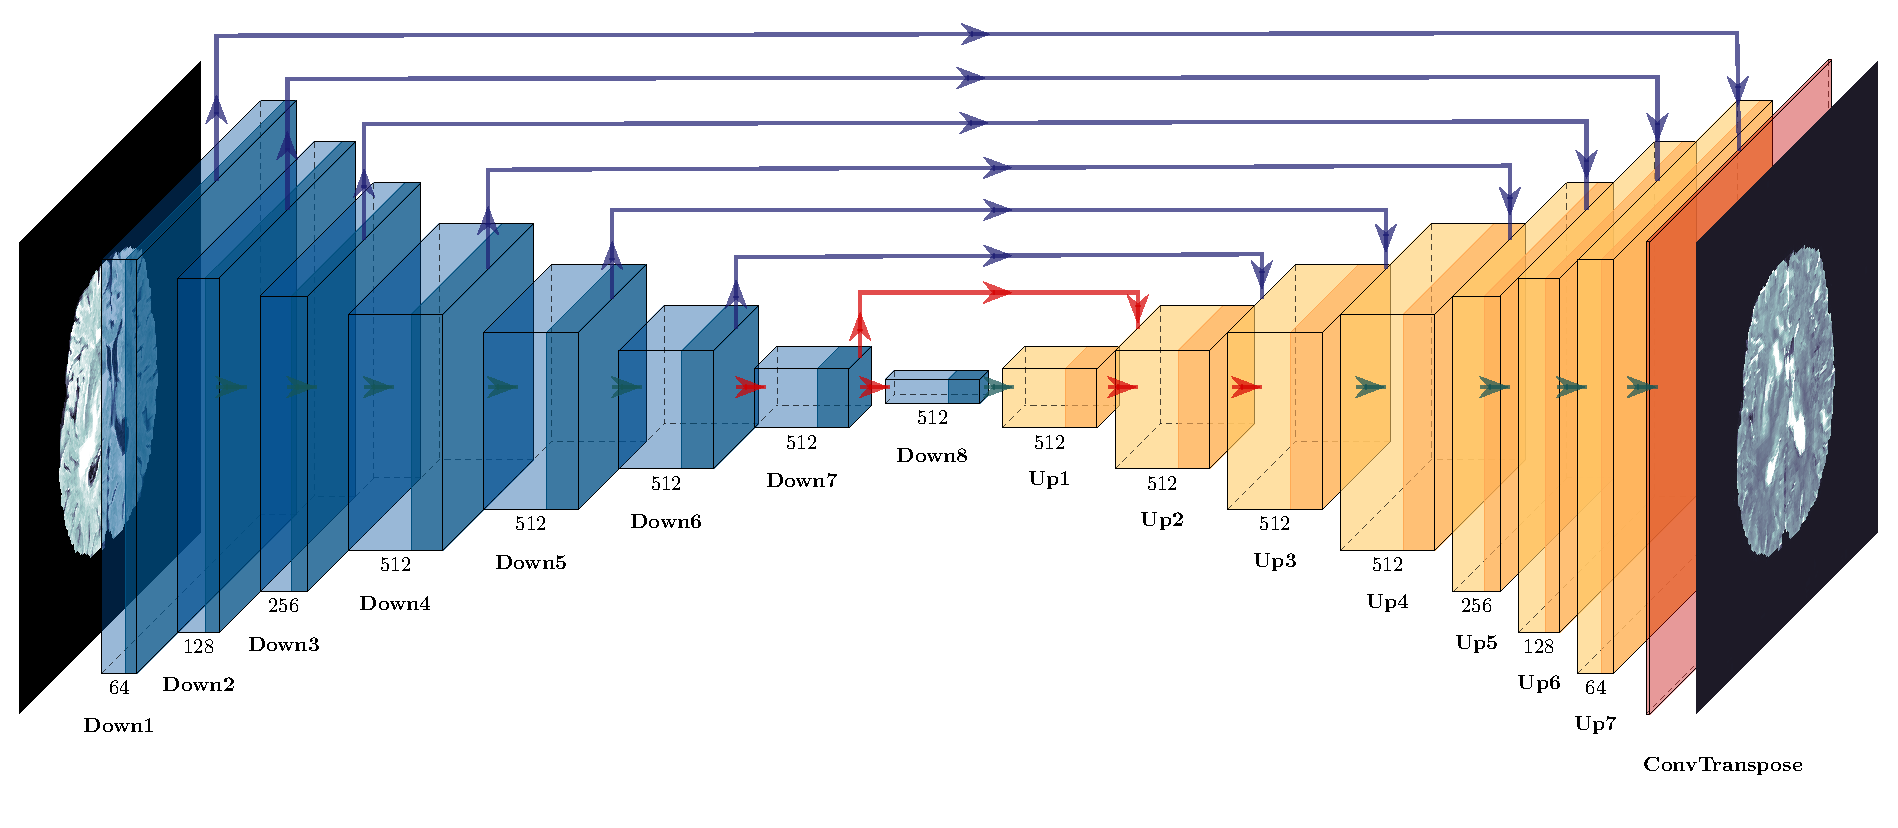
\includegraphics[height=0.266\textheight]{images/config_internal.pdf}
\caption[Configuration example in Internal Connections Analysis]{Example of network corresponding to the configuration [1,1,1,1,1,0,0] in the Internal Connections Analysis. In red the connections turned off.}
\label{fig:config_internal}
\end{figure}
\vspace{5mm}
It is worth to highlight that, even though this analysis focuses on the internal connections, when a pair of inner channels are off (except in the case of the 7th and 9th links), then also the entries of a skip connection are forced to 0, as it possible to observe in Figure \ref{fig:config_internal} where all the connections turned off are shown in red color.

%%%%%%%%%%%%%%%%  Internal connection analysis MI-p2p 
\begin{table}[H]
\centering
\fontsize{8.5}{16}\selectfont
\setlength{\tabcolsep}{4pt}
\begin{tabular}{c|c|c|c|c|c}
\toprule
\textbf{Internal off} & \textbf{MSE} & \textbf{PSNR} & \textbf{SSIM} & $\mathbf{MSE_{tumor}}$ & $\mathbf{PSNR_{tumor}}$\\
\hline

[1,1,1,1,1,1,1] & $\mathbf{0.0069\pm0.0049}$ & $\mathbf{22.8165\pm3.7317}$  & $\mathbf{0.7772\pm0.1094}$ & $\mathbf{0.0221\pm0.0375}$ & $\mathbf{19.0374\pm4.1582}$\\

[0,1,1,1,1,1,1] & $\mathrm{0.0103\pm0.0058}$ & $\mathrm{20.8939\pm3.7816}$  & $\mathrm{0.7062\pm0.1355}$ & $\mathrm{0.0406\pm0.0173}$ & $\mathrm{14.3578\pm2.0877}$\\

... & ... & ... & ... & ... & ... \\

[0,0,0,0,0,0,0] & $\mathrm{0.0103\pm0.0058}$ & $\mathrm{20.8939\pm3.7816}$  & $\mathrm{0.7062\pm0.1355}$ & $\mathrm{0.0406\pm0.0173}$ & $\mathrm{14.3578\pm2.0877}$\\
\hline
[1,1,1,1,1,1,1] & $\mathbf{0.0069\pm0.0049}$ & $\mathrm{22.8165\pm3.7317}$  & $\mathrm{0.7772\pm0.1094}$ & $\mathrm{0.0221\pm0.0375}$ & $\mathbf{19.0374\pm4.1582}$\\

[1,1,1,1,1,1,0] & $\mathbf{0.0069\pm0.0049}$ & $\mathbf{22.8750\pm3.7301}$  & $\mathbf{0.7794\pm0.1084}$ & $\mathbf{0.0218\pm0.0346}$ & $\mathrm{18.9272\pm4.0549}$\\

[1,1,1,1,1,0,0] & $\mathrm{0.0077\pm0.0048}$ & $\mathrm{22.2194\pm3.6022}$  & $\mathrm{0.7579\pm0.1165}$ & $\mathrm{0.0229\pm0.0384}$ & $\mathrm{18.4526\pm3.8248}$\\

[1,1,1,1,0,0,0] & $\mathrm{0.0095\pm0.0054}$ & $\mathrm{21.2806\pm3.7368}$  & $\mathrm{0.7505\pm0.1164}$ & $\mathrm{0.0393\pm0.0253}$ & $\mathrm{14.6543\pm2.3238}$\\

[1,1,1,0,0,0,0] & $\mathrm{0.0104\pm0.0062}$ & $\mathrm{20.8601\pm3.6599}$  & $\mathrm{0.7192\pm0.1326}$ & $\mathrm{0.0400\pm0.0454}$ & $\mathrm{15.1987\pm3.1458}$\\

[1,1,0,0,0,0,0] & $\mathrm{0.0108\pm0.0059}$ & $\mathrm{20.6812\pm3.7336}$  & $\mathrm{0.7403\pm0.1178}$ & $\mathrm{0.0444\pm0.0259}$ & $\mathrm{14.0582\pm2.2371}$\\

[1,0,0,0,0,0,0] & $\mathrm{0.0162\pm0.0086}$ & $\mathrm{18.8502\pm3.5119}$  & $\mathrm{0.6641\pm0.1233}$ & $\mathrm{0.0845\pm0.0249}$ & $\mathrm{10.9653\pm1.7048}$\\

[0,0,0,0,0,0,0] & $\mathrm{0.0103\pm0.0058}$ & $\mathrm{20.8939\pm3.7816}$  & $\mathrm{0.7062\pm0.1355}$ & $\mathrm{0.0406\pm0.0173}$ & $\mathrm{14.3578\pm2.0877}$\\
\midrule
\end{tabular}
\caption[Quantitative results from internal connections off in MI-pix2pix]{Quantitative results from the Internal Connections Analysis on MI-P2P{$_{T_{2flair}}$}: channels are sequentially turned off.}
\label{tab:quantitative_internal_off_mip2p}
\end{table}

\begin{figure}[H]
\includegraphics[width=0.635\textheight]{images/internal_mip2p.pdf}
\caption[Qualitative results from internal connections off in MI-pix2pix]{Qualitative results from the Internal Connections Analysis on MI-P2P{$_{T_{2flair}}$}: channels are sequentially turned off. \textit{Prediction} corresponds to config.[1111111]}


\centering
\label{fig:qualitative_internal_off_mip2p}
\end{figure}
\newpage
\section{Experiments Discussion}
\label{sec:experiments_discussion}
While in Subsection \ref{subsec:metrics_discussion} we demonstrated that the input received by our models isn't just outputted but it is elaborated, allowing to produce a completely new synthesized image, in Sections \ref{sec:skip_analysis} and \ref{sec:internal_analysis} we investigated about which connections, in a generator network, are used the most in this processing: in this section we discuss the results obtained from the experiments presented in the previous sections, eventually referring to the additional results reported in \autoref{cha:first_appendix}.

\vspace{5mm}
Table \ref{tab:quantitative_internal_off_mip2p}, reporting the quantitative results from the Internal Connection Analysis, shows that all the configurations with the the first (and the last, since they are turned off in pairs) internal channels off reach the exactly same performances in the evaluation metrics. This is due to the fact that all the entries of the connection between the last and the second-last layers are set to 0 and so the information coming from the input is sent to the output only through the outermost skip connection.

\vspace{5mm}
Looking at the values from Table \ref{tab:quantitative_internal_off_mip2p} it is possible to appreciate how the values in the performances don't deteriorate too much compared to the configuration with all the channels on. This is a first indicator about the importance of the skips connections in the generator networks: with all the internal connections off and with all the skips off with the exception of the outermost, the network is able to still obtain satisfiable results, with a worsening in the performance of 49\% in MSE, 8\% in PSNR, 9\% in SSIM, 84\% in $MSE_{tumor}$ and 25\% in $PSNR_{tumor}$. 

\vspace{5mm}
Observing Tables \ref{tab:quantitative_channels_off_mip2p} and \ref{tab:quantitative_channels_perturbed_mip2p} from the Skip Connection Analysis, we can confirm the major role played by the outermost skip connection in the generative process: when all the skips values are forced to 0 and the information passes only through internal connections, the network performs worse, compared to the [1111111] configuration, by a significant degradation of 1330\% in MSE, 55\% in PSNR, 97\% in SSIM, 1362\% in $MSE_{tumor}$ and 73\% in $PSNR_{tumor}$ (Figure \ref{fig:barplot_1}).

\begin{figure}
\centering
\includegraphics[width=0.635\textheight]{images/barplot_1.pdf}
\caption[Percentual degradation in the performances of MI-pix2pix]{Percentual degradation observed in the performances of MI-pix2pix, with respect to the configuration with all the connections, skips and internal, ON (Config. [1111111]).}
\label{fig:barplot_1}
\end{figure}


This degradation in the performances can be easily appreciated also by a visual comparison of the qualitative results shown in Figure \ref{fig:qualitative_channels_off_mip2p} and it reinforces the hypothesis that these connections are crucial for a generative model since they allow to recover the information lost in the contracting path through the many downsampling blocks.

\vspace{5mm}
The outermost skip is for sure the connection that brings the most significant source of information to the output image but in general, looking both at Figure \ref{fig:qualitative_channels_off_mip2p} and Table \ref{tab:quantitative_channels_off_mip2p}, we can observe how the scores obtained from the metrics drop to low values more rapidly by switching off the outer connections than switching first the inner ones, due to the fact the most external skips are crucial for a Generative Adversarial network.

\vspace{5mm}
The results we obtained in the second part (skips perturbed, Subsection \ref{subsec:skips_perturbed}) of the Skip Connections Analysis are consistent with what was observed in the first one (skips off, Subsection \ref{subsec:skips_turned_off}) and show a similar behaviour in the degradation of the performances. 
The qualitative results, instead, show even better what we said about the most external links: Figure \ref{fig:qualitative_channels_perturbed_mip2p} illustrates how the appearance belonging to the image $A$ is completely almost compromised after perturbing the generator with the replacement, in two outermost skip connections, of the content belonging to $A$ with the one produced by another network that takes as input $B$.

\vspace{5mm}
Further experiments on MI-GAN and pix2pix, that can be found in Appendix \ref{cha:first_appendix}, show that the unimodal model, compared to two multi-modal networks, seems to have more balance in the gap between the contributions of the skip connections to the generated image: the outermost skip connections remain the most significant for the generative process but to a lesser extent with respect to what we observed with the multi-input generator. 

\begin{figure}
\centering
\includegraphics[width=0.635\textheight]{images/barplot_2.pdf}
\caption[Percentual degradation in the performances of different models]{Percentual degradation observed in the performances of the different models when all the internal channels are turned off (and so every skip connections is off, except for the outermost one), with respect to the configuration with all the connections, skips and internal, ON (Config. [1111111]).}
\label{fig:barplot_2}
\end{figure}

This can be visually appreciated by a comparison between Figures \ref{fig:qualitative_channels_off_p2p} and \ref{fig:qualitative_channels_off_mip2p} but also by the quantitative results from the analysis on the internal connections, with pix2pix that, switching off all the connections except for the last skip channel, deteriorates more (238\% in MSE, 25\% in PSNR, 21\% in SSIM) than MI-pix2pix (49\% in MSE, 8\% in PSNR, 9\% in SSIM) and MI-GAN (72\% in MSE, 11\% in PSNR, 15\% in SSIM) (Figure \ref{fig:barplot_2}).


\section{Summary}
\label{sec:6th_section_summary}
In this chapter we presented the experiments conducted in order to investigate about which are the connections used the most during the generative process of the models we trained.

Then we reported and evaluated both the quantitative and the qualitative results reached with our tests, discussing the observed behaviour of the generator network and showing the insights provided by the Skip Connections Analysis and by the Internal Connections Analysis: the experiments performed led us to the conclusion that skip connections (in particular the outermost skip connections) have a crucial role in the generative process and by turning off or perturbing these channels, a significant degradation in the performances of the network is observed.

\vspace{5mm}
In the next chapter, we provide more general considerations on our work and we present the open problems as well as the possible future works.